\documentclass[a4paper,12pt]{article}
\usepackage[utf8]{inputenc}
\usepackage[spanish]{babel}
\usepackage{amsmath}
\usepackage{graphicx}
\usepackage[hidelinks]{hyperref}
\usepackage{lipsum}

\title{Algoritmo de Máquinas de Soporte Vectorial (SVM) en Minería de Datos}
\author{José Benavente}
\date{\today}

\begin{document}

\maketitle

\newpage

\tableofcontents

\newpage

\section{Introducción}
La minería de datos es una técnica para extraer conocimiento a partir de grandes volúmenes de datos. En este informe se analizará el algoritmo de \textbf{Máquinas de Soporte Vectorial (SVM)}, la cual es una herramienta eficaz para resolver problemas de clasificación y regresión en aprendizaje automático. SVM es particularmente útil en escenarios donde las clases no son linealmente separables. Para la implementación práctica de este algoritmo, se utilizará el lenguaje Python junto con la biblioteca \texttt{scikit-learn}.

\section{Descripción del algoritmo SVM}
\subsection{Teoría del Algoritmo}

Las \textbf{Máquinas de Soporte Vectorial (SVM)} son algoritmos supervisados que se utilizan para problemas de clasificación y regresión. El objetivo de SVM es encontrar un \textit{hiperplano óptimo} que separe las distintas clases en un espacio de características. Para datos linealmente separables, el hiperplano maximiza el \textit{margen} entre los puntos de datos más cercanos de cada clase, denominados \textit{vectores de soporte}.

En los casos en que las clases no son separables linealmente, SVM emplea una técnica conocida como \textit{kernel trick}, que proyecta los datos a un espacio de mayor dimensionalidad donde las clases puedan ser separadas.

\pagebreak

\subsubsection{Función de Kernel}
La función de kernel transforma los datos originales en un espacio de características de mayor dimensión, lo que permite resolver problemas no lineales. Los kernels más comunes son:

\begin{itemize}
   \item \textbf{Kernel Lineal}: El kernel lineal es el más simple de todos y no realiza ninguna transformación de los datos. En este caso, los datos se clasifican directamente en el espacio original utilizando una línea recta (o un hiperplano en dimensiones superiores).
   
  \begin{center}
    \large{$K(x, x') = x \cdot x'$}
  \end{center}

  \item \textbf{Kernel Polinómico}: El kernel polinómico eleva el producto escalar de los vectores de características a una potencia, lo que efectivamente transforma los datos a un espacio de características de mayor dimensión. Esto permite capturar relaciones más complejas entre las clases.
  
  \begin{center}
    \large{$K(x, x') = (x \cdot x' + c)^d$}
  \end{center}
  
  \item \textbf{Kernel RBF (\textit{Radial Basis Function})}: El kernel RBF, también conocido como kernel gaussiano, es uno de los más poderosos y comúnmente utilizados. Este kernel mapea los puntos de datos en el espacio original a un espacio de características de dimensión infinita, donde es más probable que los datos sean linealmente separables.
  
  \begin{center}
    \large{$K(x, x') = \exp\left(-\frac{\|x - x'\|^2}{2\sigma^2}\right)$}
  \end{center}
  
\end{itemize}

\pagebreak

\subsection{Aplicaciones}

SVM tiene una amplia gama de aplicaciones, tales como:
\begin{itemize}
    \item Clasificación de imágenes, como en el reconocimiento de dígitos manuscritos.
    \item Detección de fraudes en transacciones financieras.
    \item Bioinformática, para la clasificación de genes.
    \item Análisis de sentimientos en textos.
\end{itemize}

\subsection{Ventajas y Desventajas}

\textbf{Ventajas}:
\begin{itemize}
    \item Funciona bien en espacios de alta dimensionalidad.
    \item Eficaz en problemas donde las clases no son separables linealmente.
    \item Utiliza un subconjunto de puntos de datos (vectores de soporte), lo que lo hace eficiente en términos de memoria.
    \item Soporta diversos tipos de kernels que permiten adaptar el modelo a diferentes tipos de problemas.
\end{itemize}

\textbf{Desventajas}:
\begin{itemize}
    \item No es adecuado para conjuntos de datos extremadamente grandes debido a su costo computacional.
    \item La elección del kernel y los parámetros influye fuertemente en el desempeño.
    \item Puede ser difícil de interpretar cuando se usan kernels no lineales.
\end{itemize}

\section{Descripción de la herramienta o lenguaje de programación}

Para la implementación de SVM se utiliza \textbf{Python}, un lenguaje de programación popular en ciencia de datos y análisis de datos. En particular, la biblioteca \texttt{scikit-learn} proporciona una implementación eficiente del algoritmo SVM.

\subsection{Python y scikit-learn}
Python es un lenguaje sencillo y muy utilizado en el campo de la ciencia de datos debido a su extensa colección de bibliotecas. \texttt{scikit-learn} es una de las bibliotecas más poderosas en Python para implementar algoritmos de minería de datos y aprendizaje automático.

\section{Implementación del algoritmo en Python}

A continuación, se presenta un ejemplo de implementación del algoritmo de Máquinas de Soporte Vectorial (SVM) utilizando Python y la biblioteca \texttt{scikit-learn}.

\subsection{Instalación de librerías necesarias}

Para ejecutar este código es necesario instalar las siguientes librerías. Esto se puede hacer a través del gestor de paquetes de Python, \textbf{pip}.

\begin{verbatim}
pip install numpy pandas scikit-learn matplotlib
\end{verbatim}

\subsection{Código de Implementación}

\begin{verbatim}
import os
from datetime import datetime

import numpy as np
import pandas as pd
from sklearn.model_selection import train_test_split
from sklearn.svm import SVC
from sklearn.metrics import accuracy_score
import matplotlib.pyplot as plt
from sklearn.datasets import load_iris


def plot_decision_boundaries(X, y, model, save_path=None):
  x_min, x_max = X.iloc[:, 0].min() - 1, X.iloc[:, 0].max() + 1
  y_min, y_max = X.iloc[:, 1].min() - 1, X.iloc[:, 1].max() + 1
  xx, yy = np.meshgrid(np.arange(x_min, x_max, 0.02),
  np.arange(y_min, y_max, 0.02))
  
  Z = model.predict(np.c_[xx.ravel(), yy.ravel()])
  Z = Z.reshape(xx.shape)
  
  plt.contourf(xx, yy, Z, alpha=0.8, cmap=plt.cm.coolwarm)
  
  scatter = plt.scatter(X.iloc[:, 0], X.iloc[:, 1], c=y, 
   edgecolors='k', marker='o', s=50, cmap=plt.cm.coolwarm)
  
  handles, labels = scatter.legend_elements()
  class_labels = ['Setosa', 'Versicolor']
  plt.legend(handles, class_labels, title="Especies")
  
  plt.xlabel('Longitud del Sepal (cm)')
  plt.ylabel('Anchura del Sepal (cm)')
  plt.title('Clasificación de Flores Iris')
  
  if save_path:
  plt.savefig(save_path, format='png', dpi=500)
  
  plt.show()


def main():
  data = load_iris()
  df = pd.DataFrame(data.data, columns=data.feature_names)
  df['target'] = data.target
  
  df = df[df['target'] != 2]
  X = df[['sepal length (cm)', 'sepal width (cm)']]
  y = df['target']
  
  X_train, X_test, y_train, y_test = train_test_split(X,
   y, test_size=0.3, random_state=42)
  
  svm_model = SVC(kernel='rbf', gamma='auto')
  svm_model.fit(X_train, y_train)
  
  y_pred = svm_model.predict(X_test)
  
  accuracy = accuracy_score(y_test, y_pred)
  print(f'Precision del modelo SVM: {accuracy * 100:.2f}%')
  
  timestamp = datetime.now().strftime("%Y%m%d_%H%M%S")
  save_dir = "plots"
  os.makedirs(save_dir, exist_ok=True)
  save_path = os.path.join(save_dir,
   f"svm_decision_boundary_{timestamp}.png")
  
  plot_decision_boundaries(X_test, y_test, svm_model, save_path)


if __name__ == "__main__":
  main()
\end{verbatim}

\subsection{Explicación del Código}
\begin{itemize}
    \item \textbf{Carga de datos}: Se utiliza el conjunto de datos \textit{Iris}, que es conocido en problemas de clasificación.
    \item \textbf{División del conjunto de datos}: Los datos se dividen en un conjunto de entrenamiento y un conjunto de prueba con una proporción 70\%-30\%.
    \item \textbf{Modelo SVM}: Se crea un modelo SVM con un kernel lineal, aunque se pueden usar otros kernels dependiendo de la naturaleza de los datos.
    \item \textbf{Entrenamiento}: Se entrena el modelo con los datos de entrenamiento.
    \item \textbf{Evaluación}: Se evalúa la precisión del modelo usando los datos de prueba.
\end{itemize}

\pagebreak

\subsection{Resultado de la Ejecución del Código}

Al ejecutar el código anteriormente descrito, podemos ver un gráfico el cual tiene la siguiente lógica: de las tres clases de flor que originalmente maneja Iris, se seleccionan dos de ellas para esta demostración, la ''Setosa'' y la ''Versicolor'', cada una representada por los puntos del gráfico. Los ejes del gráfico hacen referencia a la anchura de la flor, y la longitud de la flor, y la linea que hay en medio de ambos grupos representa el hiperplano.

\begin{center}
  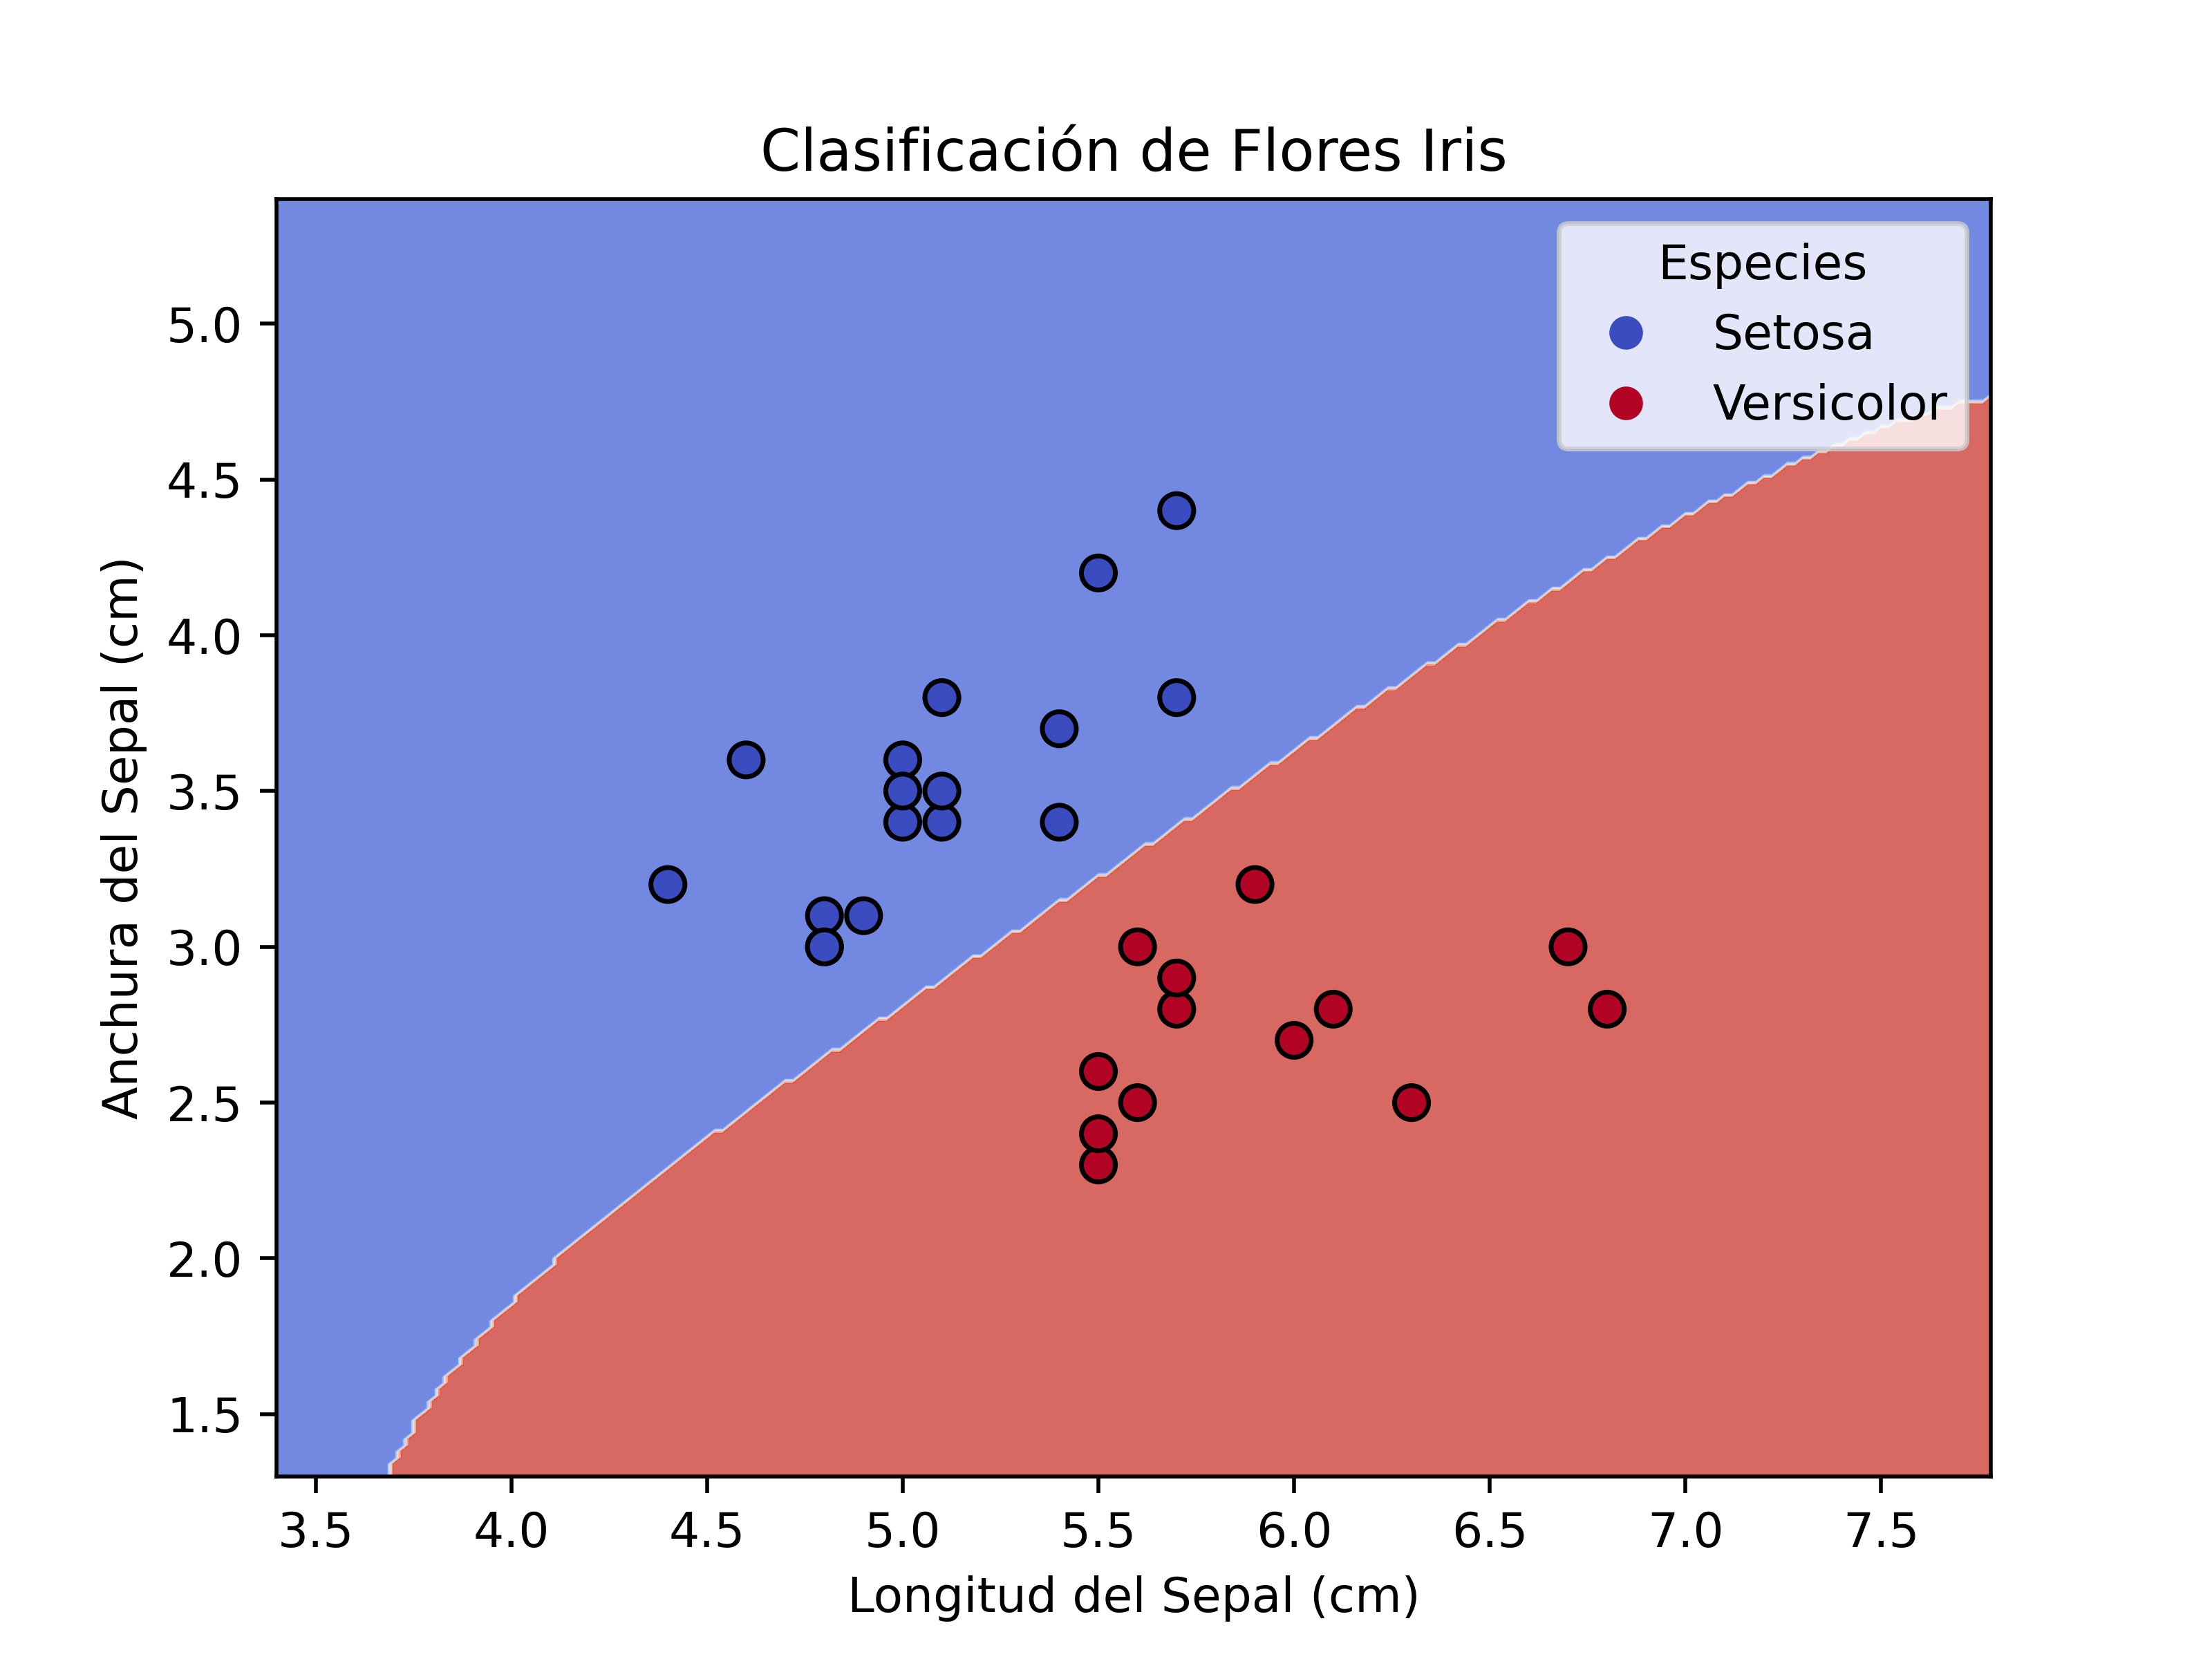
\includegraphics[width=10cm, height=10cm]{plots/svm_decision_boundary_20241011_222144.png}
\end{center}

Este gráfico busca responder a lo siguiente: ''Dados el ancho y la longitud de cierta clase de flor, ¿qué tan probable es que ésta sea de la especie Setosa o Versicolor?. El clasificador SVM no solo está viendo las propiedades de las flores (ancho y largo), sino que también está intentando aprender la relación entre estas dos propiedades y los tipos de flor.

Una vez aprende esta relación, crea el límite de decisión, el cual es una línea o región que separa el espacio en áreas en donde se predice una clase versus la otra. Eso es lo que se ve en el gráfico con regiones coloreadas en base a las predicciones del clasificador para las clases Setosa y Versicolor. Por lo tanto, en este caso, la precisión fue de un 100\%.

\section{Conclusiones}
En este informe se ha descrito el algoritmo de \textbf{Máquinas de Soporte Vectorial (SVM)} y su implementación en Python utilizando la biblioteca \texttt{scikit-learn}.

SVM es un algoritmo robusto y eficaz para problemas de clasificación y regresión, y su flexibilidad para trabajar con datos linealmente no separables lo hace especialmente valioso en escenarios complejos. Sin embargo, es importante optimizar los parámetros del kernel para garantizar un rendimiento adecuado.

\end{document}
